\documentclass[Thesis.tex]{subfiles}
\begin{document}
%
\chapter{Augmented Monte Carlo Localization in six dimensions}
%
%\section{The algorithm}
%
\begin{algorithm}[!htp]

\caption{AMCL6D}
\label{alg:amcl6d}

\SetKwFunction{mm}{motion\mathunderscore model}
\SetKwFunction{sm}{sensor\mathunderscore model}
\SetKwFunction{ev}{evaluation}
\SetKwFunction{rsrand}{resample\mathunderscore random}
\SetKwFunction{rsclose}{resample\mathunderscore close}
\SetKwFunction{sort}{sort}
\SetKwFunction{rand}{rand}
\SetKwData{rval}{random}

\SetKwProg{amcl}{AMCL6D}{}{end}

\amcl{$(X_{t-1}, u_{t}, m_{t})$} {

\BlankLine

\tcc{Initialize}
$X_t$ = $X_{t-1}$\;
init $\theta_{rand}$, $\theta_{close}$, $\theta_{prob}$\;

\BlankLine

\tcc{Update motion and sensor model}
\ForEach{$x \in X_{t}$}{ 
  $x.pose$ = \mm{$x.pose, u_{t}$}\;
  $x.raytrace$ = \sm{$x.pose$}\;
  $x.likelihood$ = \ev{$x.raytrace, m_{t}$}\;
}

\BlankLine

\tcc{Find normalization constant $\eta$}
$\eta = \frac{1}{ \sum\limits_{X_{t}}{\left( x.likelihood\ \cdot\ x.probability\right) } }$\;\label{alg:geteta}

\BlankLine

\tcc{Calculate posterior probabilities}
\ForEach{$x \in X_{t}$}{
  $x.probability = \eta \cdot x.likelihood\ \cdot\ x.probability$\;
}

\BlankLine

\tcc{Resampling}
\sort{$X_{t}$}\;

\ForEach{$x \in X_{t} \wedge x \notin X_{t,best}$}{
  \rval = \rand{}\;
  \uIf{\rval $< 1-\theta_{rand}$}{
    $x$ = \rsrand{}\;
  }
  \uElseIf{\rval $< 1-\theta_{close}$}{
    $x$ = \rsclose{$x, X_t$}\;
  }
  \ElseIf{$x.probability < \theta_{prob}$}{
    $x$ = \rsrand{}\;
  }
}

\Return{$X_t$}

\BlankLine
}

\end{algorithm}
Mobile robots have to work in 3D environments. Such environments can be represented by continuous maps in which robots need to be able to locate themselves. The algorithm \glsreset{AMCL6D}\gls{AMCL6D} is designed to solve the localization problem in this kind of maps.

\gls{AMCL6D} is a modification of the \gls{AMCL} algorithm presented in \cite{ThrunBurgardFox:2005}. Three major components are changed: The motion model, the sensor model, and the evaluation function. The motion model (\algRef{alg:motionmodel}) supports motion in six dimensions and updates the pose samples accordingly. The sensor model (\algRef{alg:sensormodel}) is implemented by a ray trace algorithm. This sensor model allows for simulated scan values in the 3D polygon map. Simulated scans are needed for the last changed major component, the evaluation function (\algRef{alg:eval}). The evaluation function employs a \gls{knn} algorithm to determine the average distance of the real sensor data to the sensor model. Additionally the sample respawn mechanism was slightly modified. Instead of keeping a varying amount of samples depending on the overall likelihood, a static amount of samples is kept. However, if new samples need to be spawned, some of them are spawned close to samples with high beliefs instead of being spawned randomly.

Before the iterative \gls{AMCL6D} algorithm starts, the program generates $n$ random samples $X_{t=0}$. They are uniformly distributed across the map, as described in \secRef{sec:init_samples}. Initially every sample gets assigned with a probability of $\nicefrac{1}{n}$. As soon as some motion is detected, \algRef{alg:amcl6d} starts the first iteration and updates the samples $X_{t-1}$ to $X_{t}$.

The update procedure consists of several steps. First the motion model (\algRef{alg:motionmodel}) will be applied to each sample, moving them according to the detected motion. After that, each sample's sensor model needs to be updated. This is done by ray traces as described in \algRef{alg:sensormodel}. The ray tracer can be adjusted to match any kind of distance sensors, and it has to be adjusted accordingly. The results from the ray traces get evaluated to derive the likelihood for each sample.

The samples' likelihoods and their probabilities are used to calculate their posterior probabilities. Before the last step the samples are sorted according to their posterior probabilities. Their order determines if and how they are respawned: The unlikeliest samples are discarded and for each of them a new sample is generated.

\smallskip

The algorithm has three input parameters. First the samples from the last time step $X_{t-1}$, which will be updated to $X_t$ during the algorithm. Each sample $x \in X_t$ has a pose ($x.pose$), a probability ($x.probability$), a likelihood ($x.likelihood$), and a point cloud ($x.raytrace$). The pose and the probability are initialized during the sample generation, while the likelihood and point cloud get assigned later.

To update the samples according to the motion model, the robot motion $u_{t}$ between times $t-1$ and $t$ is needed. This is usually supplied by odometry data. The last input parameter is the measured sensor input $m_{t}$ in form of a point cloud, that is a collection of points which get compared to the sensor model simulation.

Additionally to the input parameters there are a few global parameters to tweak the algorithm, namely $\theta_{rand}$, $\theta_{close}$, and $\theta_{prob}$. They are thresholds used to determine which samples get regenerated and how.
%
%
%
%
%
%
\section{Motion model}\label{sec:motion_model_section}
%
\begin{algorithm}[!htp]
\caption{Motion model}
\label{alg:motionmodel}

\SetKwFunction{genNoise}{generate\mathunderscore noise}
\SetKwData{noise}{noise}
\SetKwProg{mm}{motion\mathunderscore model}{}{end}
\mm{$(x.pose, u_{t})$}{
  \noise = \genNoise{$\Sigma$}\;
  $x.pose.position += u_{t}.position + $\noise$\left[0 \dots 2\right]$\;
  $q_{yaw} =$ new QuaternionAboutAxis(ZAxis, \noise$\left[3\right]$)\;
  $q_{pitch} =$ new QuaternionAboutAxis(YAxis, \noise$\left[4\right]$)\;
  $q_{roll} =$ new QuaternionAboutAxis(XAxis, \noise$\left[5\right]$)\;
  $x.pose.orientation = q_{roll} \cdot q_{pitch} \cdot q_{yaw} \cdot u_{t}.orientation^{-1} \cdot x.pose.orientation$\;
  \Return{$x.pose$}\;
}
\end{algorithm}
%
Real sensors are subject to noise. Whenever a robot moves or turns around, its odometry data will have some errors.
To update the pose samples accordingly, the motion model in \algRef{alg:motionmodel} has to describe these uncertainties as well.

Therefor it makes use of a covariance matrix $\Sigma$, which stores how the error values of the sensors are related to each other. There are different relations for every robot, so the correct values have to be estimated or determined empirically.
%\todo[inline]{a covariance matrix and some explanations how to read it}

After any arbitrary time step the pose samples have to be updated according to the robot's movement, i.e. the motion model. It adds the difference between the start and goal pose (i.e. the movement) to the current pose and additionally some noise values which are drawn from a multivariate normal distribution. The distribution is around the origin and its variances are taken from the covariance matrix $\Sigma$ mentioned above. 

An illustration can be found at the 2D example in \figRef{fig:2d_noise_sampling}. The initial pose $p_{t-1}$ at time $t-1$ gets updated with the motion $\Delta p$ and the noise drawn from the normal distribution. It is more likely for the final pose $p_t$ to be close to the original motion.
\begin{figure}[!htp]
  \todo[inline]{add picture}
  \caption[2D motion model]{The motion model updates the pose sample $p$ by adding the motion $\Delta p$ and some normal distributed noise (using the identity matrix $I$ as deviations). The resulting pose is more likely in the red area.}
  \label{fig:2d_noise_sampling}
\end{figure}
%
Since multivariate normal distributions do not have analytical \glspl{cdf} (which could be inverted to sample from them), one has to use some other techniques to sample from them. A very common approach is described by James E. Gentle\cite{Gentle:2005}. It generates samples with the following formula:
%
\begin{align}
n = C^T z + \mu \label{form:mvndsampling}
\end{align}

Here $z$ is a vector of \gls{iid} random values drawn from one dimensional standard normal distributions. The vector $z$ gets right-multiplied to the matrix $C^T$, which is the Cholesky factorization of the covariance matrix (such that $C^TC = \Sigma$). This adjusts the sampled values to fit the multivariate normal distribution. Lastly, the $\mu$-vector gets added in order to shift the means to the correct positions.

Contrary to the classical \gls{AMCL}, in \gls{AMCL6D} not only three but six random values are drawn for each pose sample. The first three values simply get added to the position: $(x_t, y_t, z_t)^T = (x_{t-1}, y_{t-1}, z_{t-1})^T + \Delta p + (n_1, n_2, n_3)^T$, where $n_1$ describes the first element of the vector $n$, the sampled noise.
Since the robot's covariance matrix uses Euler angles but the orientations are handled by quaternions, the values for the rotation can not simply be added. Instead they are used to create new quaternions $q_{yaw}, q_{pitch},$ and $q_{roll}$ to express rotations about the yaw, pitch and roll axes respectively (in \algRef{alg:motionmodel} the \gls{ROS} coordinate system is used). These three rotations get multiplied with the updated orientation (that is $q_{t-1}$ rotated by the inverse of the orientation difference $\Delta q^{-1}$): $q_{t} = q_{roll} \cdot q_{pitch} \cdot q_{yaw} \cdot \Delta q^{-1} \cdot q_{t-1}$. Note that quaternion multiplication is non-commutative, so the order is important: The right-most rotation is done first. This order of rotations results in the traditional three body rotation inspired in aviation: First an airplane is able to yaw, when it starts it pitches and in the air it is additionally able to roll.

Putting the position and orientation together the pose sample for time $t$ is updated with the correct noise values.
%
%
%
%
%
%
\section{Sensor model}\label{sec:sensormodel}
%
\begin{algorithm}[!htp]
\caption{Sensor model}
\label{alg:sensormodel}

\SetKwData{raytrace}{raytrace}
\SetKwFunction{rtAt}{raytrace\mathunderscore at}
\SetKwFunction{normRT}{normalize\mathunderscore raytrace}
\SetKwProg{sm}{sensor\mathunderscore model}{}{end}
\sm{$(x.pose)$}{
  \raytrace = \rtAt{$x.pose$}\;
  \raytrace = \normRT{\raytrace, $x.pose$}\;
  \Return{\raytrace}\;
}
\end{algorithm}
%
The sensor model, illustrated in \algRef{alg:sensormodel}, is an exchangeable component of \gls{AMCL}. \gls{AMCL6D} is working on continuous polygon maps, which require a suiting form of sensor models. For \gls{AMCL6D} the sensor model is implemented as a ray tracer. This allows to simulate accurate sensor data in the form of point clouds in continuous maps. 

%\subsection{Ray tracing}
\label{sec:raytrace}
The ray tracer used in \gls{AMCL6D} calculates the intersections of rays emanating from the robot's position with the map. Since laser scanners, cameras, or other sensors do not only emit a single light ray, the ray tracer for \gls{AMCL6D} also needs to test many rays. 

Since the rays are supposed to simulate a camera, they are cast through an image plane. This helps to determine a second point to construct the rays: The image plane will be divided into small cells, depending on the simulated resolution. One ray is cast through each of these cells and for each of them it has to be checked whether it intersects with the map or not. If it does, the intersection point is stored into a point cloud. The ray tracing is illustrated in \figRef{fig:raytrace_scheme}.
%
\begin{figure}[!htp]
  \todo[inline]{add picture}
  %\includegraphics[width=\columnwidth]{pics/raytrace_scheme}
  \caption[Ray tracing]{Rays are cast from the robot's position through the image plane.}
  \label{fig:raytrace_scheme}
\end{figure}
%
The image plane is calculated with the aperture angles ($\theta$ for the horizontal and $\phi$ for the vertical aperture angle, measured in radians) and the focal length ($F$) of the simulated sensor. It is described by the intersections of its four edges and gets divided into cells according to the horizontal and vertical resolution of the sensor. To calculate the intersections in the virtual image plane, the following formulas are used.
%
\begin{align}
y_{min} &= F \cdot \tan{-\frac{\theta}{2}} &\label{form:image_plane} \\
y_{max} &= F \cdot \tan{ \frac{\theta}{2}} &\\
z_{min} &= F \cdot \tan{-\frac{\phi}{2}} &\\
z_{max} &= F \cdot \tan{ \frac{\phi}{2}} &
\end{align}
%
Thus, the image plane's corners are $c_{bl}=(y_{min}, z_{min}), c_{br}=(y_{max}, z_{min}), c_{tl}=(y_{min}, z_{max}),$ and $c_{tr}=(y_{max}, z_{max})$. The cell size ($w$idth and $h$eight) is calculated with $w=|c_{br}-c_{bl}|/res_{hor}$ and $h=|c_{tl}-c_{bl}|/res_{ver}$, with $res_{hor}$ being the horizontal and $res_{ver}$ the vertical resolution.

However, algorithmically it is not necessary to calculate all these points or individual cells. $y_{min/max}, z_{min/max}$ and the cell size of the image plane's cells, $w$ and $h$, are already enough to iterate over the plane and cast a ray for each cell with \algRef{alg:iterate_imageplane}. The resulting intersections are stored into an array of points which is called point cloud.
%
\begin{algorithm}[!htp]
\caption[Ray tracing]{Iterating the virtual image plane to cast rays through each cell.}
\label{alg:iterate_imageplane}
$y = y_{min}$\;
$z = z_{min}$\;
\While{$y \le y_{max}$}{
  \While{$z \le z_{max}$}{
    cast ray from $pose.position$ through $(y,z)$, store intersection\;
    $z += h$\;
  }
  $y += w$\;
}
\end{algorithm}

To speed up the intersection checks, the \gls{CGAL} offers the ability to build an \gls{AABB}\label{page:aabb} from the map data\cite{cgal:atw-aabb-14b}. The \gls{AABB} stores the mesh faces of the polygon map in axis-aligned bounding boxes. Axis-aligned bounding boxes are cuboids with all their edges parallel to the corresponding axis of the global coordinate system. They \gls{AABB} organizes them in a tree structure, this makes it faster to process the data. 
The speed up is achieved by checking for an intersection of the ray with a bounding box before calculating the exact intersection with the encased geometry. Additionally the fact that the bounding boxes are axis-aligned helps with the speed up, it allows for only simple predicate calls\cite{cgal:atw-aabb-14b}.
\begin{figure}%
  \centering
  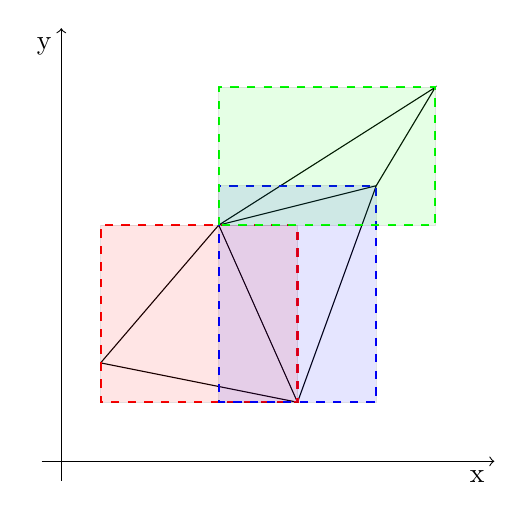
\begin{tikzpicture}[scale=5]
  % axes
	\draw[thin, <->] (1.1,0) node[below left]{x} -| (0, 1.1) node[below left]{y};
  \draw[thin, -] (-0.05,0) -| (0,-0.05);
  
  % mesh
  \coordinate (A) at (0.1, 0.25);
  \coordinate (B) at (0.6, 0.15);
  \coordinate (C) at (0.4, 0.6);
  
  \coordinate (D) at (0.8, 0.7);
  
  \coordinate (E) at (0.95, 0.95);
  
  \draw[thin, -] (A) -- (B) -- (C) -- (A);
  \draw[thin, -] (C) -- (D) -- (B);
  \draw[thin, -] (C) -- (E) -- (D);
  
  %\fill[red] (A) circle(.2pt);
  %\fill[red] (B) circle(.2pt);
  %\fill[red] (C) circle(.2pt);
  %\fill[red] (D) circle(.2pt);
  %\fill[red] (E) circle(.2pt);
  
  % bounding boxes (fill not elegant, but need to get it done)
  \draw[thick, dashed, red]     (A) |- (B) |- (C) -| (A);
  \draw[fill=red, opacity=.1]   (A) |- (B) |- (C) -| (A);
  \draw[thick, dashed, blue]    (C) |- (D) |- (B) -| (C);
  \draw[fill=blue, opacity=.1]  (C) |- (D) |- (B) -| (C);
  \draw[thick, dashed, green]   (C) |- (E) |- (C);
  \draw[fill=green, opacity=.1] (C) |- (E) |- (C);
\end{tikzpicture}
  \caption[Axis-aligned bounding boxes]{Axis-aligned bounding boxes encasing a simple mesh consisting of three triangles.}%
  \label{fig:aabb_ex}%
\end{figure}
%
\figRef{fig:raytrace} pictures an example ray trace showing the simulated robot's pose (arrow) and the point cloud which resulted from the ray trace at that pose.
\begin{figure}[!htp]
  \centering
  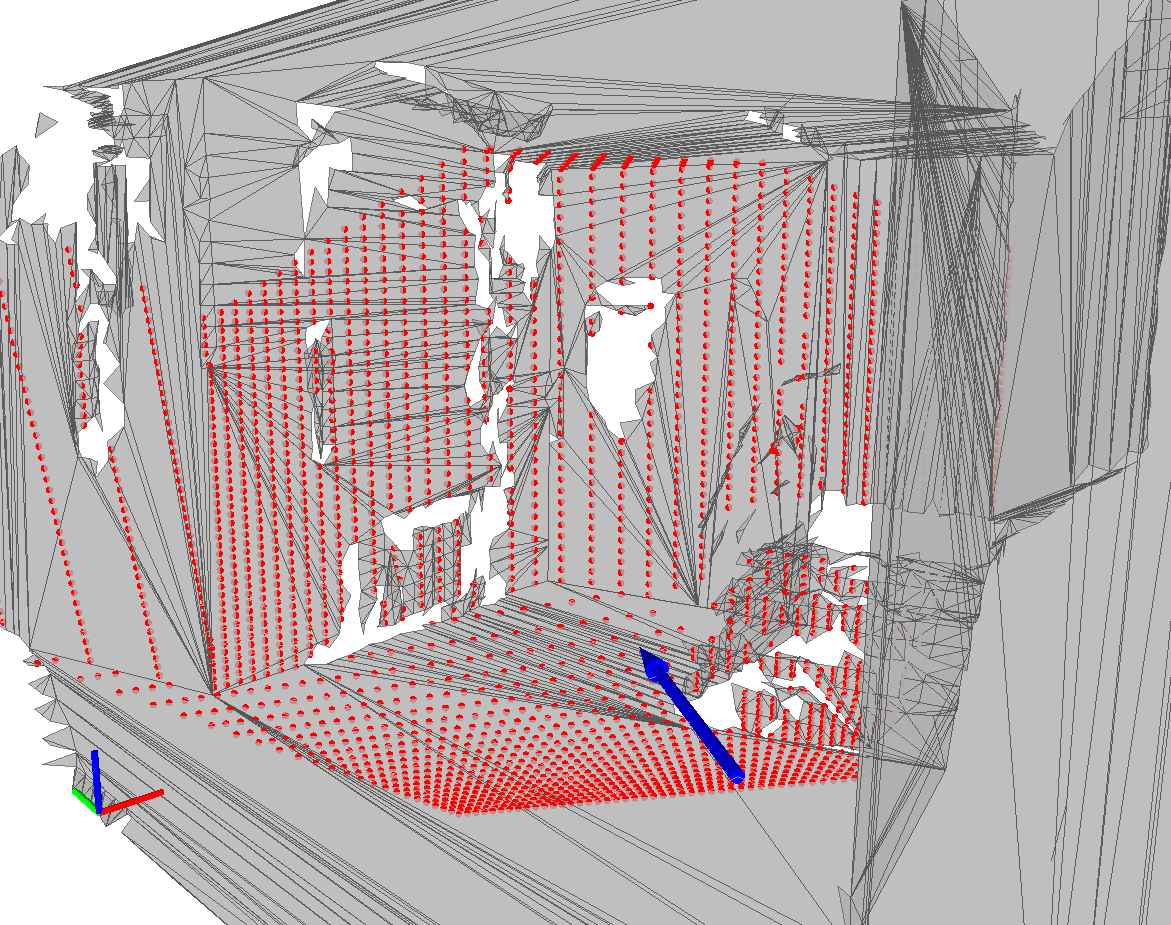
\includegraphics[width=.75\columnwidth]{pics/example_raytrace}
  \caption[Sample ray trace]{A simulated ray trace sample.}
  \label{fig:raytrace}
\end{figure}
%
To be able to compare the point cloud generated by the ray trace with the point cloud from the sensor, they need to be in the same reference frame. This means they both have to be transformed in a way such that their origins are at the same point. \gls{AMCL6D} uses the global origin.
To transform a pose to the origin, it is possible to use an affine transformation matrix. This affine transformation matrix $A$ can be constructed easily: The orientation of the pose can be expressed by a $3\times3$ rotation matrix $R$ and the translation by a $3\times1$ matrix $T$. These two matrices can be combined and extended to a $4\times4$ matrix (\formRef{form:affinetransmatrix}).
\begin{align}
A = \left(\begin{array}{cccc}
      R_{1,1} & R_{1,2} & R_{1,3} & T_{1,1} \\ 
      R_{2,1} & R_{2,2} & R_{2,3} & T_{2,1} \\ 
      R_{3,1} & R_{3,2} & R_{3,3} & T_{3,1} \\
         0    &    0    &    0    &    1
    \end{array}\right)\label{form:affinetransmatrix}
\end{align}
$A$ is the matrix which describes the transformation needed from the global origin to the pose. By taking the inverse $A^{-1}$ it is possible to calculate a matrix which describes the opposite: the transformation from the pose back to the origin. This inverted matrix $A^{-1}$ can be applied to each point $p$ in the point cloud result ($\mathbb{P}$) from the ray trace to transform them to positions which are relative to the origin as they were to the pose. Note that the points need to be homogenous, that means they need to be extended with a fourth component which is $1$.
%
\begin{align}
  \forall p \in \mathbb{P}: \genfrac{(}{)}{0pt}{0}{p}{1} = A^{-1} \genfrac{(}{)}{0pt}{0}{p}{1}
\end{align}
%
The resulting point cloud can be used to evaluate the corresponding sample in the evaluation function.
%
%
%
\section{Evaluation function}
%
\begin{algorithm}[!htp]
\caption{Sample evaluation}
\label{alg:eval}
\SetKwFunction{kd}{prepare\mathunderscore kd\mathunderscore tree}
\SetKwFunction{knn}{k\mathunderscore nearest\mathunderscore neighbors}
\SetKwFunction{ed}{euclidean\mathunderscore distance}
\SetKwFunction{size}{size}
\SetKwData{kdtree}{kd\mathunderscore tree}
\SetKwData{nn}{nearest\mathunderscore neighbor}
\SetKwData{avgdst}{average\mathunderscore distance}
\SetKwProg{ev}{evaluation}{}{end}
\SetKwData{smallval}{$\epsilon$}

\ev{$(x.raytrace, m_t)$}{
  \kdtree = \kd{$x.raytrace$}\;
  \avgdst = \smallval\;
  \ForEach{$p \in m_t$}{
    \nn = \knn{$p$, \kdtree, 1}\;
    \avgdst += \ed{$p$, \nn} / \size{$m_t$}\;
  }
  \Return{1/\avgdst}
}
\end{algorithm}
The likelihood for each sample gets calculated in the evaluation function (\algRef{alg:eval}). Most of it is done with the \gls{FLANN}. First the sample's point cloud gets organized into a \gls{kdtree}. In the second step a \gls{knn} search is performed for each point in the sensor measurements to determine each respective closest neighbor. 

A \gls{kdtree} is a binary tree structure which recursively splits the space and stores each subspace into a child node of the previous one. Thus the root node resembles the whole space and the first split plane, its child nodes contain the subspaces yielded by the split plane. This is done until there is only one point left in a subspace, which becomes a leaf node. 

The \gls{knn} algorithm is used to find similarities in high dimensional data\cite{flann_pami_2014}. Its purpose is to find the $k$ points of a dataset which are closest to a given point. The most naive version of such an algorithm would just iterate over all points to search the $k$ closest points, \gls{FLANN} takes advantage of the \gls{kdtree} to speed up the calculations. 
In \gls{AMCL6D} the \gls{knn} algorithm is used as a heuristic to find the distance to the closest point ($k=1$) in the simulated sensor data for each point in the real sensor data. For each sample the mean distance to the real data is calculated.

By inverting the mean distance between the real sensor data and a sample it is possible to come up with a value between $0$ and $1$. This value is inverse proportional to the distance, that means if the distance is huge the value becomes really small, but if the distance is small the value gets closer to $1$. To avoid division by zero in the unlikely but possible case that the measurements have a distance of $0$, the average distance gets initialized with an arbitrary small value $\epsilon \in \mathbb{R} > 0$.

The result of the evaluation function is used as the likelihood for the calculation of a sample's new probability: $x.probability_t = \eta \cdot x.likelihood \cdot x.probability_{t-1}$. $\eta$ is the normalization constant, which is the marginalization over all posterior probabilities (see \lineRef{alg:amcl6d}{alg:geteta}).
After evaluating the samples, they are sorted by their posterior probabilities. This allows for easier regeneration of poses with low posterior beliefs.


\end{document}